\section{The local halo}\label{sec:1.2}

Every rate in this book is an average over the dark matter that passes through the detector. That average is fixed by the local mass density, which sets how many particles there are, and by the velocity distribution in the laboratory, which sets how fast they move and from which direction they come.

\subsection{Density and velocity distribution}

Measurements of the local dark-matter density, from the motion of stars near the Sun and from the rotation curve of the Galaxy, give values between 0.2 and \SI{0.6}{GeV.cm^{-3}}~\cite[Sect.~3.1.1]{baxter2021recommended}. Mass models with different halo shapes and data sets disagree by more than their statistical errors~\cite[Sect.~3.1]{green2012astrophysical}. For this reason direct-detection results are quoted for a fixed reference value; we use the recommended one~\cite[Table~1]{baxter2021recommended},
\begin{equation}
  \rho_\chi = \SI{0.3}{GeV.cm^{-3}} = \SI{2.31e-6}{eV^4},
  \label{eq:1.2-rho}
\end{equation}
where the value in natural units follows from multiplying by $(\hbar c)^3$, with $\hbar c = \SI{1.973e-5}{eV.cm}$ (\cref{app:A.1}). Since the density enters every rate as an overall factor, a different value rescales a limit without changing its shape~\cite[Sect.~3.1.1]{baxter2021recommended}. The number density of particles of mass $m_\chi$ is $\nd_\chi = \rho_\chi/m_\chi$: three particles per cubic centimeter at \SI{100}{MeV}, three thousand at \SI{100}{keV}. For comparison, \SI{0.3}{GeV.cm^{-3}} is the mass of one hydrogen atom in roughly \SI{3}{cm^3}, while a crystal holds about $10^{23}$ atoms in each cubic centimeter.

The velocity distribution is modeled first in the rest frame of the Galaxy, in which the halo as a whole does not rotate. We write $\vect{v}_{\mathrm{gal}}$ for a dark-matter velocity in that frame and use Cartesian galactic axes: the first points from the Sun to the Galactic center, the second along the direction of Galactic rotation, and the third to the north Galactic pole~\cite[Sect.~5]{green2012astrophysical}. The \emph{standard halo model} (SHM) takes the halo to be a singular isothermal sphere, a self-gravitating gas with density $\rho_{\mathrm{halo}}(r) \propto r^{-2}$ at galactocentric radius $r$, which encloses a mass growing linearly with $r$ and so gives the flat rotation curve of \cref{sec:1.1}~\cite[Sect.~2.1]{green2012astrophysical}. Its particles have an isotropic Maxwellian distribution,
\begin{equation}
  f_{\mathrm{gal}}(\vect{v}_{\mathrm{gal}}) = \frac{1}{N_{\mathrm{esc}}}\, \ee^{-v_{\mathrm{gal}}^2/v_0^2}\, \Theta(v_{\mathrm{esc}} - v_{\mathrm{gal}}),
  \label{eq:1.2-fgal}
\end{equation}
normalized to $\int \dd^3 v_{\mathrm{gal}}\, f_{\mathrm{gal}} = 1$, with $v_{\mathrm{gal}} = |\vect{v}_{\mathrm{gal}}|$ and $\Theta(x)$ the Heaviside step function~\cite[Eq.~(10)]{baxter2021recommended}. It is specified by the speed parameter $v_0$ and the escape speed $v_{\mathrm{esc}}$, which together fix the normalization $N_{\mathrm{esc}}$.

The speed parameter $v_0$ is the local circular speed. Each Cartesian component of $\vect{v}_{\mathrm{gal}}$ in \cref{eq:1.2-fgal} has variance $v_0^2/2$, and for $\rho_{\mathrm{halo}} \propto r^{-2}$ the Jeans equation, which balances the gradient of the velocity pressure $\rho_{\mathrm{halo}} v_0^2/2$ against gravity, gives $v_0 = v_{\mathrm{c}}$~\cite[Eq.~(11)]{green2012astrophysical}. We take the speed of the local standard of rest, the circular orbit at the Sun's radius, $v_0 = \SI{238}{km.s^{-1}}$ (\cref{tab:1-shm}).

The escape speed $v_{\mathrm{esc}}$ truncates the distribution. A particle faster than the local escape speed is not bound to the Galaxy and is assumed absent. Since the isothermal sphere itself has an infinite escape speed, the cut is imposed by hand, and the sharp step is an idealization~\cite[Sect.~2.1]{green2012astrophysical}. The value $v_{\mathrm{esc}} = \SI{544}{km.s^{-1}}$ comes from the fastest stars in the Radial Velocity Experiment (RAVE) survey; later surveys give medians from 485 to \SI{580}{km.s^{-1}}~\cite[Sect.~3.1.2 and Table~2]{baxter2021recommended}.

The normalization $N_{\mathrm{esc}}$ follows in spherical coordinates~\cite[Eq.~(15)]{griffin2018directional}. Since the integrand depends only on $v_{\mathrm{gal}}$, the angles contribute $4\pi$, and
\begin{equation}
  N_{\mathrm{esc}} = 4\pi \int_0^{v_{\mathrm{esc}}} \dd y\, y^2 \ee^{-y^2/v_0^2}
  = \pi^{3/2} v_0^3 \left[\operatorname{erf}\!\left(\frac{v_{\mathrm{esc}}}{v_0}\right) - \frac{2}{\sqrt{\pi}}\,\frac{v_{\mathrm{esc}}}{v_0}\, \ee^{-v_{\mathrm{esc}}^2/v_0^2}\right],
  \label{eq:1.2-nesc}
\end{equation}
with the error function $\operatorname{erf}(x) = (2/\sqrt{\pi})\int_0^x \ee^{-y^2}\dd y$ (\cref{app:C.8}). The second equality integrates $y^2 \ee^{-y^2/v_0^2}$ once by parts; \cref{app:D.1} writes the step out. Without the cut, $N_{\mathrm{esc}}$ would be the Gaussian integral $\pi^{3/2}v_0^3$; the bracket is the fraction of that Gaussian below $v_{\mathrm{esc}}$.

The Sun moves through this distribution. Its velocity in the galactic frame is the circular velocity of the local standard of rest plus the Sun's peculiar motion relative to it~\cite[Table~1 and Eq.~(14)]{baxter2021recommended},
\begin{equation}
  \vect{v}_{\odot} = (0, 238, 0) + (11.1, 12.2, 7.3)\ \si{km.s^{-1}} = (11.1, 250.2, 7.3)\ \si{km.s^{-1}},
  \label{eq:1.2-vsun}
\end{equation}
in the galactic axes above. The magnitude is $|\vect{v}_{\odot}| = (11.1^2 + 250.2^2 + 7.3^2)^{1/2}\,\si{km.s^{-1}} = \SI{250.55}{km.s^{-1}}$, which we round to the reference value $\SI{250.5}{km.s^{-1}}$. \Cref{tab:1-shm} collects the parameters.

\begin{table}[t]
  \centering
  \caption{Standard-halo-model parameters adopted in this book, with their sources. Vectors are given in galactic axes (toward the Galactic center, along Galactic rotation, toward the north Galactic pole). The last two rows follow from the others. The reference Earth speed is the adopted magnitude of the solar velocity $(0, 238, 0) + (11.1, 12.2, 7.3)$\,\si{km.s^{-1}}. The largest laboratory speed adds it to the escape speed.}
  \label{tab:1-shm}
  \begin{tabular}{@{}llll@{}}
    \toprule
    Symbol & Quantity & Value & Source \\
    \midrule
    $\rho_\chi$ & local dark-matter density & \SI{0.3}{GeV.cm^{-3}} & \cite[Table~1]{baxter2021recommended} \\
    $v_0$ & circular speed at the Sun's radius & \SI{238}{km.s^{-1}} & \cite[Table~1]{baxter2021recommended} \\
    $v_{\mathrm{esc}}$ & Galactic escape speed & \SI{544}{km.s^{-1}} & \cite[Table~1]{baxter2021recommended} \\
    -- & solar peculiar velocity & $(11.1, 12.2, 7.3)$\,\si{km.s^{-1}} & \cite[Table~1]{baxter2021recommended} \\
    -- & mean orbital speed of the Earth & \SI{29.8}{km.s^{-1}} & \cite[Eq.~(13)]{baxter2021recommended} \\
    $\vect{v}_\oplus(t)$ & Earth velocity relative to the Sun & \cref{eq:1.2-vorb} & \cite[Eq.~(11)]{baxter2021recommended} \\
    $v_{\mathrm{E}}^{\mathrm{ref}}$ & reference Earth speed (adopted $|\vect{v}_\odot|$) & \SI{250.5}{km.s^{-1}} & \cref{eq:1.2-vsun} \\
    $v_{\mathrm{max}}$ & largest laboratory speed $v_{\mathrm{esc}} + v_{\mathrm{E}}^{\mathrm{ref}}$ & \SI{794.5}{km.s^{-1}} & \cref{eq:1.2-vmax} \\
    \bottomrule
  \end{tabular}
\end{table}

\subsection{The laboratory frame}

A detector shares the motion of the Earth. Its velocity in the galactic frame is
\begin{equation}
  \vect{v}_{\mathrm{E}}(t) = \vect{v}_{\odot} + \vect{v}_{\oplus}(t),
  \label{eq:1.2-vE}
\end{equation}
where $\vect{v}_{\oplus}(t)$ is the Earth's orbital velocity relative to the Sun. Since galactic speeds are below $10^{-2}$ in natural units, the change of frame is Galilean, with relativistic corrections of relative size $v^2 \approx 10^{-6}$. A particle with laboratory velocity $\vect{v}$ has galactic velocity
\begin{equation}
  \vect{v}_{\mathrm{gal}} = \vect{v} + \vect{v}_{\mathrm{E}}(t).
  \label{eq:1.2-galilean}
\end{equation}
The shift has unit Jacobian, $\dd^3 v_{\mathrm{gal}} = \dd^3 v$, and a velocity cell holds the same number of particles in both frames. The laboratory distribution is the galactic one of \cref{eq:1.2-fgal}~\cite[Eq.~(10)]{baxter2021recommended} evaluated at the boosted velocity, $f_\chi(\vect{v}) = f_{\mathrm{gal}}(\vect{v} + \vect{v}_{\mathrm{E}}(t))$:
\begin{equation}
  f_\chi(\vect{v}, t) = \frac{1}{N_{\mathrm{esc}}}\, \ee^{-|\vect{v} + \vect{v}_{\mathrm{E}}(t)|^2/v_0^2}\, \Theta\bigl(v_{\mathrm{esc}} - |\vect{v} + \vect{v}_{\mathrm{E}}(t)|\bigr).
  \label{eq:1.2-flab}
\end{equation}
We write $f_\chi(\vect{v})$ when the time is not needed, and $v = |\vect{v}|$ for the laboratory speed. The normalization is unchanged, $\int\dd^3 v\, f_\chi = 1$, and we write angle brackets for an average over the distribution, $\langle\cdots\rangle = \int \dd^3 v\, f_\chi(\vect{v})\,(\cdots)$. In the laboratory the distribution is no longer centered on zero: the most probable velocity is $-\vect{v}_{\mathrm{E}}$. Dark matter arrives as a wind from the direction in which the Earth moves. Because $f_{\mathrm{gal}}$ is even in $\vect{v}_{\mathrm{gal}}$, its mean velocity vanishes, and by \cref{eq:1.2-galilean} the mean laboratory velocity is exactly $\langle\vect{v}\rangle = -\vect{v}_{\mathrm{E}}(t)$, cut or no cut.

The spread about this mean is the galactic one: $\langle v_{\mathrm{gal}}^2\rangle^{1/2} = (3/2)^{1/2} v_0 = \SI{291}{km.s^{-1}}$ for the Gaussian and \SI{284}{km.s^{-1}} with the cut. The spread is larger than the drift: the wind is broad. A numerical integration of \cref{eq:1.2-flab} at $v_{\mathrm{E}} = v_{\mathrm{E}}^{\mathrm{ref}}$ shows that \SI{94}{\percent} of the particles move with a positive component along $-\vect{v}_{\mathrm{E}}$, and \SI{59}{\percent} within $45^\circ$ of it; the mean cosine of the angle to $-\vect{v}_{\mathrm{E}}$ is 0.66.

The fastest particle in the laboratory is one that moves at $v_{\mathrm{esc}}$ in the galactic frame, opposite to $\vect{v}_{\mathrm{E}}$; its laboratory speed is $v_{\mathrm{esc}} + |\vect{v}_{\mathrm{E}}(t)|$. We quote thresholds and kinematic edges at a fixed reference speed, the rounded solar speed $v_{\mathrm{E}}^{\mathrm{ref}} = \SI{250.5}{km.s^{-1}}$ (\cref{eq:1.2-vsun}; \cref{app:A.8}). The \emph{maximum speed} is then
\begin{equation}
  v_{\mathrm{max}} = v_{\mathrm{esc}} + v_{\mathrm{E}}^{\mathrm{ref}} = \SI{794.5}{km.s^{-1}} = 2.650\times10^{-3}.
  \label{eq:1.2-vmax}
\end{equation}
Over a year $v_{\mathrm{esc}} + |\vect{v}_{\mathrm{E}}(t)|$ ranges from 781 to \SI{810}{km.s^{-1}} (see the annual modulation below). With the reference value, thresholds stay time-independent, while integrals over $f_\chi$ use the full $\vect{v}_{\mathrm{E}}(t)$, averaged over the exposure.

Many rates depend only on the speed. The \emph{speed distribution} $F_\chi(v)$, normalized to $\int_0^\infty \dd v\, F_\chi = 1$, is $v^2$ times the integral of $f_\chi$ over directions. Take the polar axis along $\vect{v}_{\mathrm{E}}$, write $\vartheta$ for the angle between $\vect{v}$ and $\vect{v}_{\mathrm{E}}$, and $v_{\mathrm{E}} = |\vect{v}_{\mathrm{E}}|$. Then $|\vect{v} + \vect{v}_{\mathrm{E}}|^2 = v^2 + v_{\mathrm{E}}^2 + 2 v v_{\mathrm{E}} \cos\vartheta$, and the azimuth contributes $2\pi$:
\begin{equation*}
  F_\chi(v) = \frac{2\pi v^2}{N_{\mathrm{esc}}}\, \ee^{-(v^2 + v_{\mathrm{E}}^2)/v_0^2} \int_{-1}^{\cos\vartheta_{\mathrm{cut}}} \dd (\cos\vartheta)\, \ee^{-2 v v_{\mathrm{E}} \cos\vartheta/v_0^2}.
\end{equation*}
The upper limit $\cos\vartheta_{\mathrm{cut}}$ is where $|\vect{v} + \vect{v}_{\mathrm{E}}| = v_{\mathrm{esc}}$, or 1 if that never happens. For $v < v_{\mathrm{esc}} - v_{\mathrm{E}}$ no direction reaches the cut and $\cos\vartheta_{\mathrm{cut}} = 1$. For $v_{\mathrm{esc}} - v_{\mathrm{E}} < v < v_{\mathrm{esc}} + v_{\mathrm{E}}$ the cut removes the directions close to $\vect{v}_{\mathrm{E}}$, and at $\cos\vartheta_{\mathrm{cut}}$ the exponent equals $-v_{\mathrm{esc}}^2/v_0^2$. Doing the elementary integral, we find
\begin{equation}
  F_\chi(v) = \frac{\pi v_0^2\, v}{v_{\mathrm{E}} N_{\mathrm{esc}}} \times
  \begin{cases}
    \ee^{-(v - v_{\mathrm{E}})^2/v_0^2} - \ee^{-(v + v_{\mathrm{E}})^2/v_0^2}, & v < v_{\mathrm{esc}} - v_{\mathrm{E}},\\[2pt]
    \ee^{-(v - v_{\mathrm{E}})^2/v_0^2} - \ee^{-v_{\mathrm{esc}}^2/v_0^2}, & v_{\mathrm{esc}} - v_{\mathrm{E}} < v < v_{\mathrm{esc}} + v_{\mathrm{E}}
  \end{cases},
  \label{eq:1.2-Fspeed}
\end{equation}
and $F_\chi = 0$ above $v_{\mathrm{esc}} + v_{\mathrm{E}}$. The two branches join continuously at $v = v_{\mathrm{esc}} - v_{\mathrm{E}}$, and the second vanishes at $v_{\mathrm{esc}} + v_{\mathrm{E}}$. \Cref{eq:1.2-Fspeed} assumes $v_{\mathrm{E}} < v_{\mathrm{esc}}$, which holds by a factor of two. \Cref{fig:1-speed} shows $F_\chi$ on the days of largest and smallest Earth speed. In the galactic frame the speed distribution $4\pi v_{\mathrm{gal}}^2 f_{\mathrm{gal}}$ peaks at $v_0$; in the laboratory the drift moves the peak to \SI{335}{km.s^{-1}} (at $v_{\mathrm{E}} = v_{\mathrm{E}}^{\mathrm{ref}}$) and stretches the tail to $v_{\mathrm{esc}} + v_{\mathrm{E}}$.

\begin{figure}[tbp]
  \centering
  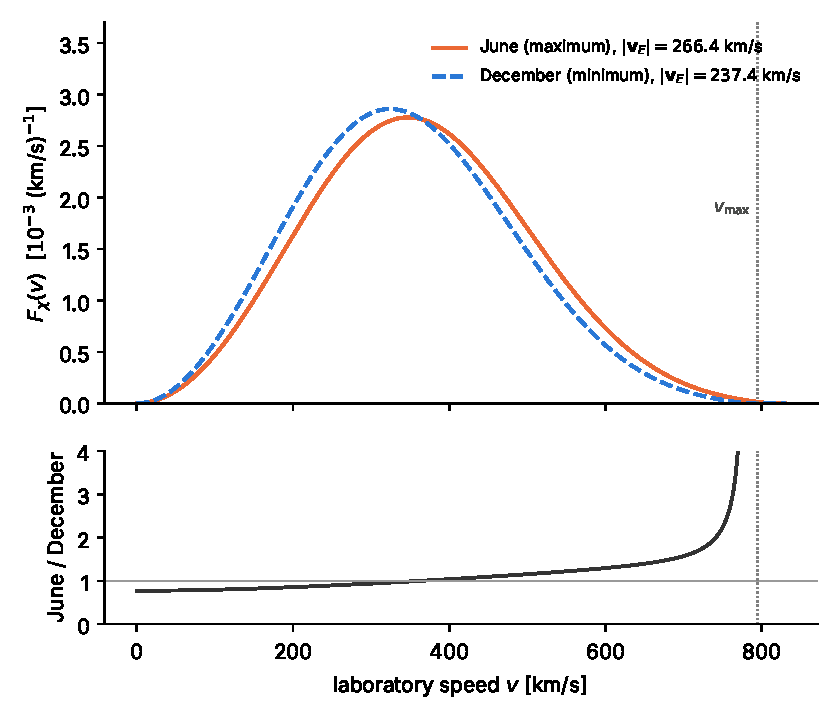
\includegraphics[width=0.85\linewidth]{figures/ch01/fig1_3.pdf}
  \caption{Top: laboratory-frame speed distribution $F_\chi(v)$ of the standard halo model with $v_0 = \SI{238}{km.s^{-1}}$ and $v_{\mathrm{esc}} = \SI{544}{km.s^{-1}}$, in June (solid, Earth speed at its annual maximum \SI{266.4}{km.s^{-1}}) and December (dashed, \SI{237.4}{km.s^{-1}}), the days of largest and smallest Earth speed for the Earth velocity of \cref{eq:1.2-vorb}~\cite[Eq.~(11)]{baxter2021recommended}. Bottom: ratio of the June to the December distribution. The dotted line marks $v_{\mathrm{max}} = \SI{794.5}{km.s^{-1}}$; in June the distribution extends to \SI{810}{km.s^{-1}}, in December to \SI{781}{km.s^{-1}}.}
  \label{fig:1-speed}
\end{figure}

The tail of $F_\chi$ matters for light dark matter, which must often use the fastest particles to deposit enough energy (\cref{sec:1.3}). We integrate \cref{eq:1.2-Fspeed} numerically at $v_{\mathrm{E}} = v_{\mathrm{E}}^{\mathrm{ref}}$. The fraction of particles faster than 400, 500, 600 and \SI{700}{km.s^{-1}} is \SI{36}{\percent}, \SI{15}{\percent}, \SI{4.2}{\percent} and \SI{0.58}{\percent}; above \SI{750}{km.s^{-1}} it is \SI{0.10}{\percent}. A threshold that needs $v \gtrsim \SI{700}{km.s^{-1}}$ sees a rate suppressed by more than two orders of magnitude, and one that depends on $v_{\mathrm{esc}}$ and on the exact shape of the cut, the most uncertain parts of the model.

Scattering rates contain the speed through $1/v$: the energy-conservation delta function of a collision, integrated over the direction of $\vect{v}$, leaves a factor $1/v$ (\cref{sec:1.3}). In the SHM this average has a closed form.

\begin{workedexample}{Normalization and mean inverse speed}\label{we:1-nesc}
With $v_{\mathrm{esc}}/v_0 = 544/238 = 2.286$, the error function is $\operatorname{erf}(2.286) = 0.99877$ and the second term in the bracket of \cref{eq:1.2-nesc} is $(2/\sqrt{\pi})(2.286)\,\ee^{-5.224} = 2.579 \times 0.005383 = 0.01388$. The bracket is $0.98489$: the cut removes \SI{1.5}{\percent} of the Gaussian. With $\pi^{3/2} v_0^3 = 5.5683 \times (238)^3\,\si{(km/s)^3} = \SI{7.507e7}{(km/s)^3}$,
\begin{equation*}
  N_{\mathrm{esc}} = 0.98489 \times \SI{7.507e7}{(km/s)^3} = \SI{7.393e7}{(km/s)^3}.
\end{equation*}
The mean inverse speed is $\langle 1/v\rangle = \int_0^\infty \dd v\, F_\chi(v)/v$. Dividing \cref{eq:1.2-Fspeed} by $v$ leaves Gaussians in $v \mp v_{\mathrm{E}}$ and a constant. Substituting $y = v - v_{\mathrm{E}}$ in the first exponential and $y = v + v_{\mathrm{E}}$ in the second, the two cancel on $v_{\mathrm{E}} < y < v_{\mathrm{esc}}$ and leave $\int_{-v_{\mathrm{E}}}^{v_{\mathrm{E}}} \ee^{-y^2/v_0^2}\dd y = \sqrt{\pi}\, v_0 \operatorname{erf}(v_{\mathrm{E}}/v_0)$; the constant term, integrated over an interval of length $2v_{\mathrm{E}}$, contributes $-2 v_{\mathrm{E}} \ee^{-v_{\mathrm{esc}}^2/v_0^2}$ (\cref{app:D.1}). Hence
\begin{equation}
  \left\langle \frac{1}{v} \right\rangle = \frac{\pi v_0^2}{v_{\mathrm{E}} N_{\mathrm{esc}}} \left[\sqrt{\pi}\, v_0 \operatorname{erf}\!\left(\frac{v_{\mathrm{E}}}{v_0}\right) - 2 v_{\mathrm{E}}\, \ee^{-v_{\mathrm{esc}}^2/v_0^2}\right].
  \label{eq:1.2-inv}
\end{equation}
At $v_{\mathrm{E}} = v_{\mathrm{E}}^{\mathrm{ref}} = \SI{250.5}{km.s^{-1}}$, $v_{\mathrm{E}}/v_0 = 1.0525$ and $\operatorname{erf}(1.0525) = 0.86338$. The bracket is $\sqrt{\pi} \times 238 \times 0.86338 - 2 \times 250.5 \times 0.005383 = 364.21 - 2.70 = \SI{361.51}{km.s^{-1}}$, and the prefactor is $\pi (238)^2/(250.5 \times \SI{7.393e7}{}) = \SI{9.608e-6}{(km/s)^{-2}}$. The result is
\begin{equation*}
  \left\langle \frac{1}{v} \right\rangle = \SI{3.474e-3}{(km/s)^{-1}} = \frac{1}{\SI{287.9}{km.s^{-1}}}, \quad\text{or } 1041 \text{ in natural units}.
\end{equation*} Without the cut, \cref{eq:1.2-inv} reduces to $\operatorname{erf}(v_{\mathrm{E}}/v_0)/v_{\mathrm{E}} = 1/(\SI{290.1}{km.s^{-1}})$; the cut removes fast particles and raises $\langle 1/v\rangle$ by \SI{0.8}{\percent}. In June and December the same formula yields $1/(\SI{298.3}{km.s^{-1}})$ and $1/(\SI{279.8}{km.s^{-1}})$, a \SI{6}{\percent} swing.
\end{workedexample}

The mean inverse speed is the value at zero of the function $\eta(\vmin) = \langle \Theta(v - \vmin)/v\rangle$ that \cref{sec:1.3} introduces, with $\vmin$ the minimum velocity of \cref{eq:1.3-vmin}; \cref{app:D.1} gives $\eta$ for every $\vmin$.

\subsection{Annual modulation}

The Earth's orbital velocity, in the galactic axes of \cref{eq:1.2-vsun}, is~\cite[Eq.~(11)]{baxter2021recommended}
\begin{equation}
  \vect{v}_{\oplus}(t) = \SI{29.8}{km.s^{-1}} \left[\begin{pmatrix} 0.9941\\ 0.1088\\ 0.0042 \end{pmatrix} \cos \omega_{\mathrm{yr}} t + \begin{pmatrix} -0.0504\\ 0.4946\\ -0.8677 \end{pmatrix} \sin \omega_{\mathrm{yr}} t \right],
  \label{eq:1.2-vorb}
\end{equation}
with $\omega_{\mathrm{yr}} = \SI{0.0172}{d^{-1}}$ the orbital angular frequency and $t$ counted in days from 22 March. The two column vectors are orthogonal unit vectors, to $10^{-4}$, that span the plane of the orbit, and \SI{29.8}{km.s^{-1}} is the mean orbital speed~\cite[Eq.~(13)]{baxter2021recommended}. We treat the orbit as a circle; its eccentricity moves the date of the largest Earth speed by 1.2 days and the modulation amplitude by \SI{0.4}{\percent}~\cite[Table~I]{mccabe2014earth}, both too small to matter here.

Since the orbital speed is small next to the solar speed, $29.8/250.5 = 0.12$, we can expand the Earth's speed to first order in it:
\begin{equation*}
  |\vect{v}_{\mathrm{E}}(t)| = \bigl(|\vect{v}_\odot|^2 + 2\vect{v}_\odot\cdot\vect{v}_\oplus + |\vect{v}_\oplus|^2\bigr)^{1/2} \approx v_{\mathrm{E}}^{\mathrm{ref}} + \hat{\vect{v}}_\odot \cdot \vect{v}_\oplus(t),
\end{equation*}
with $\hat{\vect{v}}_\odot = \vect{v}_\odot/|\vect{v}_\odot| = (0.0443, 0.9986, 0.0291)$ from \cref{eq:1.2-vsun}. Projected onto $\hat{\vect{v}}_\odot$, the two vectors of \cref{eq:1.2-vorb} have components $0.1528$ and $0.4664$, and
\begin{equation}
  |\vect{v}_{\mathrm{E}}(t)| \approx v_{\mathrm{E}}^{\mathrm{ref}} + \SI{14.6}{km.s^{-1}} \cos\bigl[\omega_{\mathrm{yr}}(t - t_{\mathrm{peak}})\bigr],
  \label{eq:1.2-annual}
\end{equation}
with amplitude $29.8 \times (0.1528^2 + 0.4664^2)^{1/2} = 29.8 \times 0.4908 = \SI{14.6}{km.s^{-1}}$ and phase $\omega_{\mathrm{yr}} t_{\mathrm{peak}} = \arctan(0.4664/0.1528) = 71.9^\circ = \SI{1.254}{rad}$, which is $t_{\mathrm{peak}} = 72.9$ days after 22 March, that is, 2 June. Only half of the orbital speed modulates the Earth's speed because the Sun's velocity makes an angle of $\arccos 0.4908 = 60.6^\circ$ with the plane of the orbit. The second-order term, $(|\vect{v}_\oplus|^2 - (\hat{\vect{v}}_\odot\cdot\vect{v}_\oplus)^2)/(2v_{\mathrm{E}}^{\mathrm{ref}})$, adds \SI{1.3}{km.s^{-1}} at both extremes and \SI{1.6}{km.s^{-1}} on average over the year. The exact speed from \cref{eq:1.2-vE,eq:1.2-vorb} is largest on 2 June, \SI{266.4}{km.s^{-1}}, smallest on 2 December, \SI{237.4}{km.s^{-1}}, and averages \SI{252.1}{km.s^{-1}} over the year.

The rate follows the change of $F_\chi$ with the season, and its sign depends on which speeds the process can use. In June the distribution is shifted to higher speeds: it holds more particles above \SI{364}{km.s^{-1}}, where the curves of \cref{fig:1-speed} cross, and fewer below. A rate that needs fast particles, such as one near a kinematic threshold, peaks in June. A rate that weights all speeds by $1/v$ peaks in December, since $\langle 1/v \rangle$ is \SI{6}{\percent} larger then (\cref{we:1-nesc}). For the integral $\eta(\vmin)$ of \cref{sec:1.3}, built from \cref{app:D.1}, the phase reverses at $\vmin = \SI{211}{km.s^{-1}}$; above, the modulation grows from a few percent to $+\SI{21}{\percent}$ and $\SI{-16}{\percent}$ about the reference value at $\vmin = \SI{600}{km.s^{-1}}$, and to $+\SI{42}{\percent}$ and $\SI{-28}{\percent}$ at \SI{700}{km.s^{-1}}. Averaged over the year, $\langle 1/v\rangle$ lies \SI{0.3}{\percent} below its value at $v_{\mathrm{E}}^{\mathrm{ref}}$ and agrees to $10^{-4}$ with its value at the annual-mean speed. In the tail the difference grows: at $\vmin = 600$ and \SI{700}{km.s^{-1}} the yearly average of $\eta$ exceeds its value at $v_{\mathrm{E}}^{\mathrm{ref}}$ by \SI{2.6}{\percent} and \SI{5.6}{\percent}, because $\eta$ there is a convex function of $v_{\mathrm{E}}$.

The size of the modulation follows from the closed forms by differentiation. For a rate that depends on time only through $v_{\mathrm{E}}$, \cref{eq:1.2-annual} makes the relative modulation about the yearly mean
\begin{equation*}
  (\SI{14.6}{km.s^{-1}})\,\frac{\partial \ln(\text{rate})}{\partial v_{\mathrm{E}}}\, \cos\bigl[\omega_{\mathrm{yr}}(t - t_{\mathrm{peak}})\bigr],
\end{equation*}
with the derivative taken at $v_{\mathrm{E}}^{\mathrm{ref}}$. For a rate proportional to $\langle 1/v\rangle$, write \cref{eq:1.2-inv} as $\pi v_0^2 \mathcal{I}(v_{\mathrm{E}})/(v_{\mathrm{E}} N_{\mathrm{esc}})$ with $\mathcal{I}(v_{\mathrm{E}})$ the bracket. Since $\dd \operatorname{erf}(x)/\dd x = (2/\sqrt{\pi})\ee^{-x^2}$, $\dd \mathcal{I}/\dd v_{\mathrm{E}} = 2\ee^{-v_{\mathrm{E}}^2/v_0^2} - 2\ee^{-v_{\mathrm{esc}}^2/v_0^2} = 0.6498$, and
\begin{equation*}
  \frac{\partial \ln\langle 1/v\rangle}{\partial v_{\mathrm{E}}} = -\frac{1}{v_{\mathrm{E}}} + \frac{1}{\mathcal{I}}\frac{\dd \mathcal{I}}{\dd v_{\mathrm{E}}} = -\frac{1}{250.5} + \frac{0.6498}{361.51} = \SI{-2.195e-3}{(km/s)^{-1}}.
\end{equation*}
The amplitude is $14.6 \times (-2.195\times10^{-3}) = \SI{-3.2}{\percent}$: the mean inverse speed is largest in December (\cref{we:1-nesc}).

Annual modulation is a signature because each of its features is fixed by the halo and the orbit, not by the detector. The period is one year, the phase is set by the June maximum and December minimum, the phase flips at a definite $\vmin$, and the amplitude grows toward the kinematic edge. A background would have to reproduce all four. The amplitude is also more sensitive to the shape of the speed distribution than the time-averaged rate is, and an observed modulation would test the halo model itself~\cite[Sect.~6.2]{green2012astrophysical}.

\subsection{Daily modulation}

The Earth also rotates, and a crystal fixed in the laboratory turns with it relative to $\vect{v}_{\mathrm{E}}$. The rotation speed, $2\pi \times \SI{6378}{km}/\SI{86164}{s} = \SI{0.47}{km.s^{-1}}$ at the equator and less by the cosine of the latitude elsewhere, is \SI{3}{\percent} of the annual amplitude of \cref{eq:1.2-annual} and leaves the speed distribution practically unchanged. What changes, however, is the direction from which the wind arrives in crystal axes.

The rotation is simplest in equatorial coordinates. Their Cartesian axes are fixed relative to the distant stars: the third points along the Earth's rotation axis to the north celestial pole, the first to the vernal equinox in the celestial equator, and the second completes a right-handed set. A direction on the sky is given by its \emph{declination}, the angle above the celestial equator, and its \emph{right ascension}, the angle measured eastward in the equatorial plane from the vernal equinox. Right ascension is often quoted in hours ($\SI{24}{h} = 360^\circ$). In equatorial Cartesian axes a direction has the polar angle $90^\circ$ minus its declination and the azimuth equal to its right ascension. A laboratory turns about the third axis once per sidereal day, the rotation period relative to the stars. Its \emph{meridian} is the half-plane bounded by the rotation axis that contains the local vertical, its \emph{local sidereal time} is the right ascension of that meridian, and the \emph{hour angle} of a direction is the local sidereal time minus the direction's right ascension.

The rotation from equatorial to galactic Cartesian axes is fixed by three angles: the equatorial coordinates of the north Galactic pole, right ascension $192.85948^\circ$ and declination $27.12825^\circ$, and the galactic longitude of the north celestial pole, $122.932^\circ$~\cite[App.~B, Eq.~(B3)]{mccabe2014earth}. Built from these angles, it takes a unit vector with equatorial components $(x_{\mathrm{eq}}, y_{\mathrm{eq}}, z_{\mathrm{eq}})$ to its galactic components,
\begin{equation}
  \begin{pmatrix} x_{\mathrm{gal}}\\ y_{\mathrm{gal}}\\ z_{\mathrm{gal}} \end{pmatrix}
  = \begin{pmatrix} -0.0549 & -0.8734 & -0.4838\\ 0.4941 & -0.4448 & 0.7470\\ -0.8677 & -0.1981 & 0.4560 \end{pmatrix}
  \begin{pmatrix} x_{\mathrm{eq}}\\ y_{\mathrm{eq}}\\ z_{\mathrm{eq}} \end{pmatrix}.
  \label{eq:1.2-rotation}
\end{equation}
The rows are the galactic axes in equatorial components; the first, the direction of the Galactic center, has right ascension $266.4^\circ$ and declination $-28.9^\circ$. The third column is the north celestial pole in galactic axes. Its scalar product with $\hat{\vect{v}}_\odot$ is $0.7378$, which means the solar velocity makes the angle
\begin{equation}
  \theta_{\mathrm{E}} = \arccos 0.7378 = 42.5^\circ,
  \label{eq:1.2-thetaE}
\end{equation}
with the rotation axis. The transpose of \cref{eq:1.2-rotation}, which is its inverse, takes $\hat{\vect{v}}_\odot$ to the equatorial components $(0.4657, -0.4887, 0.7378)$, that is, right ascension $\arctan(-0.4887/0.4657) + 360^\circ = 313.6^\circ =$ \SI{20.9}{h} and declination $47.5^\circ = 90^\circ - \theta_{\mathrm{E}}$, in the constellation Cygnus. The orbital motion moves this direction during the year, to declination $42.8^\circ$ in June and $52.6^\circ$ in December, so the angle to the rotation axis varies between $47.2^\circ$ and $37.4^\circ$. We use $\hat{\vect{v}}_\odot$ below; a prediction at the level of a few degrees computes the direction of $\vect{v}_{\mathrm{E}}(t)$ from \cref{eq:1.2-vE,eq:1.2-vorb} on each day, which combines the annual and daily modulations.

Let $\hat{\vect{n}}$ be an axis fixed in the laboratory, for example a crystal axis, at polar angle $\theta_{\hat{n}}$ from the north celestial pole. As the Earth turns, $\hat{\vect{n}}$ keeps its polar angle and its right ascension advances at the sidereal rate $\omega_{\mathrm{sid}} = 2\pi/(\SI{23}{h}\,\SI{56}{min}\,\SI{4}{s})$. In equatorial Cartesian axes the two unit vectors are $\hat{\vect{v}}_\odot = (\sin\theta_{\mathrm{E}}\cos\alpha_{\mathrm{E}}, \sin\theta_{\mathrm{E}}\sin\alpha_{\mathrm{E}}, \cos\theta_{\mathrm{E}})$, with $\alpha_{\mathrm{E}}$ its right ascension, and $\hat{\vect{n}}(t) = (\sin\theta_{\hat{n}}\cos\alpha_{\hat{n}}(t), \sin\theta_{\hat{n}}\sin\alpha_{\hat{n}}(t), \cos\theta_{\hat{n}})$, with $\alpha_{\hat{n}}(t) = \alpha_{\mathrm{E}} + \omega_{\mathrm{sid}}(t - t_{\mathrm{E}})$ and $t_{\mathrm{E}}$ the time at which both lie in one meridian plane. Their scalar product fixes the angle $\theta_{\mathrm{lab}}(t)$ between $\vect{v}_{\mathrm{E}}$ and the laboratory axis,
\begin{equation}
  \cos\theta_{\mathrm{lab}}(t) = \cos\theta_{\mathrm{E}}\cos\theta_{\hat{n}} + \sin\theta_{\mathrm{E}}\sin\theta_{\hat{n}} \cos\bigl[\omega_{\mathrm{sid}}(t - t_{\mathrm{E}})\bigr].
  \label{eq:1.2-angle}
\end{equation}
Over one sidereal day $\theta_{\mathrm{lab}}$ oscillates between $|\theta_{\mathrm{E}} - \theta_{\hat{n}}|$ and $\theta_{\mathrm{E}} + \theta_{\hat{n}}$ (for $\theta_{\mathrm{E}} + \theta_{\hat{n}} \le 180^\circ$). An axis along the rotation axis, $\theta_{\hat{n}} = 0$, keeps the fixed angle $\theta_{\mathrm{E}}$; an axis in the equatorial plane swings between $47.5^\circ$ and $132.5^\circ$. For the local vertical at latitude $\ell_{\mathrm{lat}}$ north, $\theta_{\hat{n}} = 90^\circ - \ell_{\mathrm{lat}}$ and $\alpha_{\hat{n}}$ is the local sidereal time. \Cref{fig:1-daily} plots \cref{eq:1.2-angle} for the vertical at four latitudes. At $45^\circ$N the angle runs from $2.5^\circ$, when Cygnus is nearly overhead and the wind comes from above, to $87.5^\circ$ twelve sidereal hours later.

A crystal is usually mounted with its axes along the local vertical and the local north and east directions. The full direction of $\hat{\vect{v}}_\odot$ in these axes follows from the same construction. The local vertical at latitude $\ell_{\mathrm{lat}}$ is $(\cos\ell_{\mathrm{lat}}\cos\alpha_{\mathrm{z}}, \cos\ell_{\mathrm{lat}}\sin\alpha_{\mathrm{z}}, \sin\ell_{\mathrm{lat}})$ in equatorial axes, with $\alpha_{\mathrm{z}}$ the local sidereal time. The local north is the derivative of this vector with respect to $\ell_{\mathrm{lat}}$, $(-\sin\ell_{\mathrm{lat}}\cos\alpha_{\mathrm{z}}, -\sin\ell_{\mathrm{lat}}\sin\alpha_{\mathrm{z}}, \cos\ell_{\mathrm{lat}})$. The local east is the unit vector $(-\sin\alpha_{\mathrm{z}}, \cos\alpha_{\mathrm{z}}, 0)$ in the direction of increasing $\alpha_{\mathrm{z}}$. With $\delta_{\mathrm{E}} = 90^\circ - \theta_{\mathrm{E}}$ the declination of $\hat{\vect{v}}_\odot$ and $h_{\mathrm{E}} = \alpha_{\mathrm{z}} - \alpha_{\mathrm{E}}$ its hour angle, the scalar products of these three vectors with $\hat{\vect{v}}_\odot$ are its components
\begin{equation}
  \begin{aligned}
    \hat{v}_{\mathrm{east}} &= -\cos\delta_{\mathrm{E}}\sin h_{\mathrm{E}},\\
    \hat{v}_{\mathrm{north}} &= \cos\ell_{\mathrm{lat}}\sin\delta_{\mathrm{E}} - \sin\ell_{\mathrm{lat}}\cos\delta_{\mathrm{E}}\cos h_{\mathrm{E}},\\
    \hat{v}_{\mathrm{up}} &= \sin\ell_{\mathrm{lat}}\sin\delta_{\mathrm{E}} + \cos\ell_{\mathrm{lat}}\cos\delta_{\mathrm{E}}\cos h_{\mathrm{E}}
  \end{aligned},
  \label{eq:1.2-local}
\end{equation}
with $h_{\mathrm{E}} = \omega_{\mathrm{sid}}(t - t_{\mathrm{E}})$ advancing at the sidereal rate. The vertical component is \cref{eq:1.2-angle} for $\theta_{\hat{n}} = 90^\circ - \ell_{\mathrm{lat}}$. At $45^\circ$N and $h_{\mathrm{E}} = 0$ the (east, north, up) components are $(0, 0.04, 1.00)$, a nearly vertical direction; six sidereal hours later, $h_{\mathrm{E}} = 90^\circ$, they are $(-0.67, 0.52, 0.52)$, toward the northwest at $31^\circ$ above the horizon. The wind arrives from the direction $\hat{\vect{v}}_\odot$; the dark-matter velocities point along $-\hat{\vect{v}}_\odot$.

\begin{figure}[tbp]
  \centering
  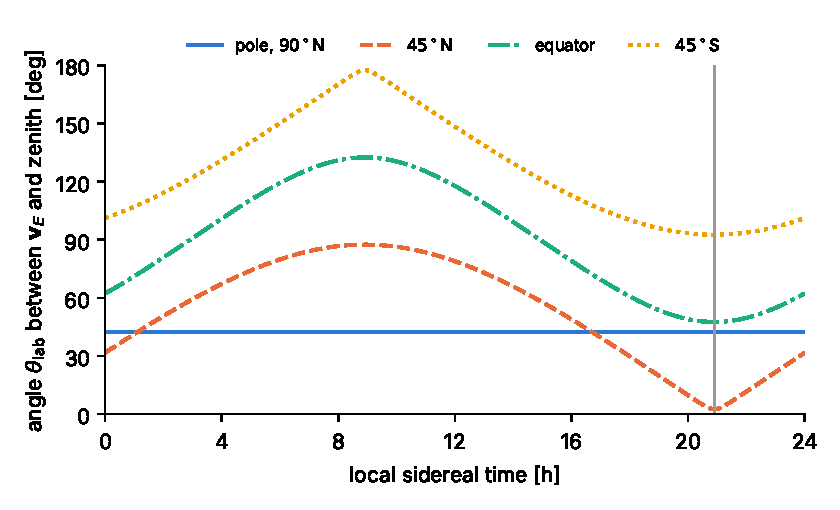
\includegraphics[width=0.85\linewidth]{figures/ch01/fig1_4.pdf}
  \caption{Angle $\theta_{\mathrm{lab}}$ between the Earth's galactic-frame velocity and the local vertical over one sidereal day, as a function of local sidereal time, at latitudes $90^\circ$N, $45^\circ$N, $0^\circ$ and $45^\circ$S. The velocity direction is that of the solar velocity, right ascension \SI{20.9}{h} and declination $47.5^\circ$ (vertical line: its transit), from Ref.~\cite[Table~1]{baxter2021recommended} and the coordinate rotation of Ref.~\cite[Eq.~(B3)]{mccabe2014earth}. The dark-matter wind arrives from this direction.}
  \label{fig:1-daily}
\end{figure}

For an isotropic target, such as a liquid or a polycrystal, the rate depends on $\vect{v}_{\mathrm{E}}$ only through its magnitude, and the rotation changes nothing. A single crystal is anisotropic: its response to a momentum transfer depends on the direction of $\vect{q}$ relative to the crystal axes, and slow dark matter transfers momentum preferentially along the wind. As $\theta_{\mathrm{lab}}$ sweeps through its daily range, the wind samples different crystal directions and the rate varies with the sidereal period.

The simplest anisotropy shows how \cref{eq:1.2-angle} enters a rate. Take a uniaxial crystal, one in which a single axis $\hat{\vect{n}}$ (the optic axis) differs from the two directions perpendicular to it, and whose response is unchanged under $\hat{\vect{n}} \to -\hat{\vect{n}}$. Since the halo of \cref{eq:1.2-flab} is symmetric under rotations about $\vect{v}_{\mathrm{E}}$, after the average over velocities the rate can depend on the two directions only through the scalar $\hat{\vect{n}}\cdot\hat{\vect{v}}_{\mathrm{E}} = \cos\theta_{\mathrm{lab}}$, and evenness in $\hat{\vect{n}}$ makes it a function of $\cos^2\theta_{\mathrm{lab}}$. To lowest order in the anisotropy the rate is a constant plus a constant times $\cos^2\theta_{\mathrm{lab}}(t)$; the crystal response fixes both constants. With the optic axis in the equatorial plane, $\theta_{\hat{n}} = 90^\circ$ and \cref{eq:1.2-angle} reduces to $\cos\theta_{\mathrm{lab}} = \sin\theta_{\mathrm{E}}\cos[\omega_{\mathrm{sid}}(t - t_{\mathrm{E}})]$; $\cos^2\theta_{\mathrm{lab}}$ then swings between 0 and $\sin^2\theta_{\mathrm{E}} = 0.456$ twice each sidereal day. With the optic axis along the Earth's axis the rate is constant.

Polar crystals, whose ions carry opposite charges, show sizable daily modulation of phonon rates when the lattice is strongly anisotropic, as in sapphire, while the cubic crystal GaAs shows almost none. The sidereal period is a distinctive signature: the sidereal day is about four minutes shorter than the solar day, and a background that follows the solar day, or does not vary at all, falls out of phase with the signal over many periods~\cite[Sect.~III\,C]{griffin2018directional}.

\subsection{Number flux}

The number flux of dark matter is the number of particles that cross a unit area per unit time. Each particle is counted across an area perpendicular to its own velocity:
\begin{equation}
  \Phi_\chi = \nd_\chi \langle v \rangle = \frac{\rho_\chi}{m_\chi}\langle v\rangle.
  \label{eq:1.2-flux}
\end{equation}
Multiplied by a velocity-independent cross-section, it is the rate per target particle. A target particle at rest presents a fixed cross-section to each incoming particle, and the particles with velocity in $\dd^3 v$ sweep a volume $v$ per unit time per unit of cross-section; they hit it at the rate $\nd_\chi f_\chi(\vect{v})\,\dd^3 v\, v$ times the cross-section. When the cross-section does not depend on $v$, summing over velocities replaces $v$ by $\langle v\rangle$, and the rate is $\Phi_\chi$ times the cross-section. When it does depend on $v$, as in most of this book, the average must be taken with the cross-section inside, and $\Phi_\chi$ serves only as a measure of how much dark matter passes through. A detector face of fixed orientation intercepts a different number, which depends on the angle between the face and the wind; \cref{eq:1.2-flux} avoids that geometric factor. The mean speed follows from \cref{eq:1.2-Fspeed} as $\langle v\rangle = \int_0^\infty \dd v\, v F_\chi(v)$. It is a sum of Gaussian moments, evaluated in \cref{app:D.1}:
\begin{equation}
  \begin{split}
  \langle v\rangle = \frac{\pi v_0^2}{v_{\mathrm{E}} N_{\mathrm{esc}}} \biggl[& v_{\mathrm{E}} v_0^2\, \ee^{-v_{\mathrm{E}}^2/v_0^2} + \sqrt{\pi}\, v_0\left(\frac{v_0^2}{2} + v_{\mathrm{E}}^2\right)\operatorname{erf}\!\left(\frac{v_{\mathrm{E}}}{v_0}\right)\\
  &- 2 v_{\mathrm{E}}\,\ee^{-v_{\mathrm{esc}}^2/v_0^2}\left(v_0^2 + v_{\mathrm{esc}}^2 + \frac{v_{\mathrm{E}}^2}{3}\right)\biggr]
  \end{split}.
  \label{eq:1.2-vmean}
\end{equation}
Without the cut ($v_{\mathrm{esc}} \to \infty$, $N_{\mathrm{esc}} \to \pi^{3/2}v_0^3$) the bracket loses its last term and \cref{eq:1.2-vmean} becomes the mean speed of a shifted Maxwellian, $v_0[\ee^{-x^2}/\sqrt{\pi} + (x + 1/(2x))\operatorname{erf}x]$ with $x = v_{\mathrm{E}}/v_0$.

\begin{workedexample}{Number flux of \SI{100}{MeV} dark matter}\label{we:1-flux}
We take $v_{\mathrm{E}} = v_{\mathrm{E}}^{\mathrm{ref}}$, so $v_{\mathrm{E}}/v_0 = 1.0525$, $\ee^{-1.1078} = 0.33028$ and $\operatorname{erf}(1.0525) = 0.86338$ (\cref{we:1-nesc}). In units of $(\si{km.s^{-1}})^3$ the three terms in the bracket of \cref{eq:1.2-vmean}, in the order written, are
\begin{align*}
  \text{first:}\quad & 250.5 \times 238^2 \times 0.33028 = \num{4.687e6},\\
  \text{second:}\quad & 1.7725 \times 238 \times (28322 + 62750) \times 0.86338 = \num{3.3170e7},\\
  \text{third:}\quad & -501 \times 0.005383 \times (56644 + 295936 + 20917) = \num{-1.0073e6}.
\end{align*}
Their sum, \num{3.6849e7}, times the prefactor \SI{9.608e-6}{(km/s)^{-2}} of \cref{we:1-nesc} gives $\langle v\rangle = \SI{354.1}{km.s^{-1}}$; without the cut it would be \SI{358.2}{km.s^{-1}}. At $m_\chi = \SI{100}{MeV}$ the number density is $\nd_\chi = (\SI{0.3}{GeV.cm^{-3}})/(\SI{0.1}{GeV}) = \SI{3}{cm^{-3}}$, so
\begin{equation*}
  \Phi_\chi = \SI{3}{cm^{-3}} \times \SI{3.541e7}{cm.s^{-1}} = \SI{1.06e8}{cm^{-2}.s^{-1}}.
\end{equation*}
About $10^8$ particles cross each square centimeter every second, $3.4\times10^{15}$ in a year. A kilogram of silicon, of density \SI{2.33}{g.cm^{-3}}, is a cube of volume \SI{429}{cm^3} and side \SI{7.5}{cm}; it holds about 1300 such particles at any instant. The flux scales as $1/m_\chi$: at \SI{1}{MeV} it is $10^{10}\,\si{cm^{-2}.s^{-1}}$. These large numbers are what makes feeble couplings testable; the cross-section, not the flux, keeps the rate small.
\end{workedexample}

\Cref{eq:1.2-flab} leaves out the gravity of the Sun and of the Earth, which bends and accelerates the particles that approach them. By energy conservation, a particle with speed $v$ far away arrives with speed $(v^2 + u_{\mathrm{esc}}^2)^{1/2}$, where $u_{\mathrm{esc}}$ is the local escape speed of the attracting body: \SI{42.1}{km.s^{-1}} from the Sun at the Earth's orbit and \SI{11.2}{km.s^{-1}} from the Earth at its surface. For $v = \SI{354}{km.s^{-1}}$ the speed increases by $u_{\mathrm{esc}}^2/2v = \SI{2.5}{km.s^{-1}}$ and \SI{0.18}{km.s^{-1}}, below \SI{1}{\percent} and comparable to the eccentricity effect; the resulting modulation from solar focusing is small~\cite[Sect.~5]{green2012astrophysical}. We neglect these shifts.

The standard halo model is a reference, not a measured distribution. Its density is uncertain by roughly a factor of two, its speed parameters by several percent, and stellar surveys reveal kinematic substructure, debris of galaxies that merged with ours, that a single Maxwellian does not describe~\cite[Sect.~3.1]{baxter2021recommended}. Near a kinematic threshold the rate probes only the tail of $F_\chi$, where these changes matter most~\cite[Sect.~6]{green2012astrophysical}. The closed form of $\eta$ in \cref{app:D.1} makes the sensitivity explicit. Changing $v_0$ by $\pm\SI{6}{km.s^{-1}}$ changes $\langle 1/v\rangle$ by $\mp \SI{1}{\percent}$, but $\eta$ at $\vmin = \SI{600}{km.s^{-1}}$ by factors 1.11 and 0.89. Changing $v_{\mathrm{esc}}$ by $\pm\SI{25}{km.s^{-1}}$ leaves $\langle 1/v\rangle$ within \SI{0.4}{\percent} and changes $\eta(\SI{600}{km.s^{-1}})$ by factors 1.06 and 0.92, but $\eta(\SI{760}{km.s^{-1}})$ by factors 2.26 and 0.10. Close to $v_{\mathrm{max}}$, the escape speed is the dominant uncertainty, larger than the annual modulation. Results in this book use the parameters of \cref{tab:1-shm}.
